%%%%\include{harmonicsexample.tex}
%\begin{figure}[ht]
%\centering
%\includegraphics[width=3.2in]{figs/harmonicsexample.pdf}
%\caption{Harmonics (courtesy: \cite{eebook}).}
%\label{fig_harmonicsexample}
%\end{figure}
\begin{figure*}[h]
	\centering{
    \begin{tabular}{cc}	
	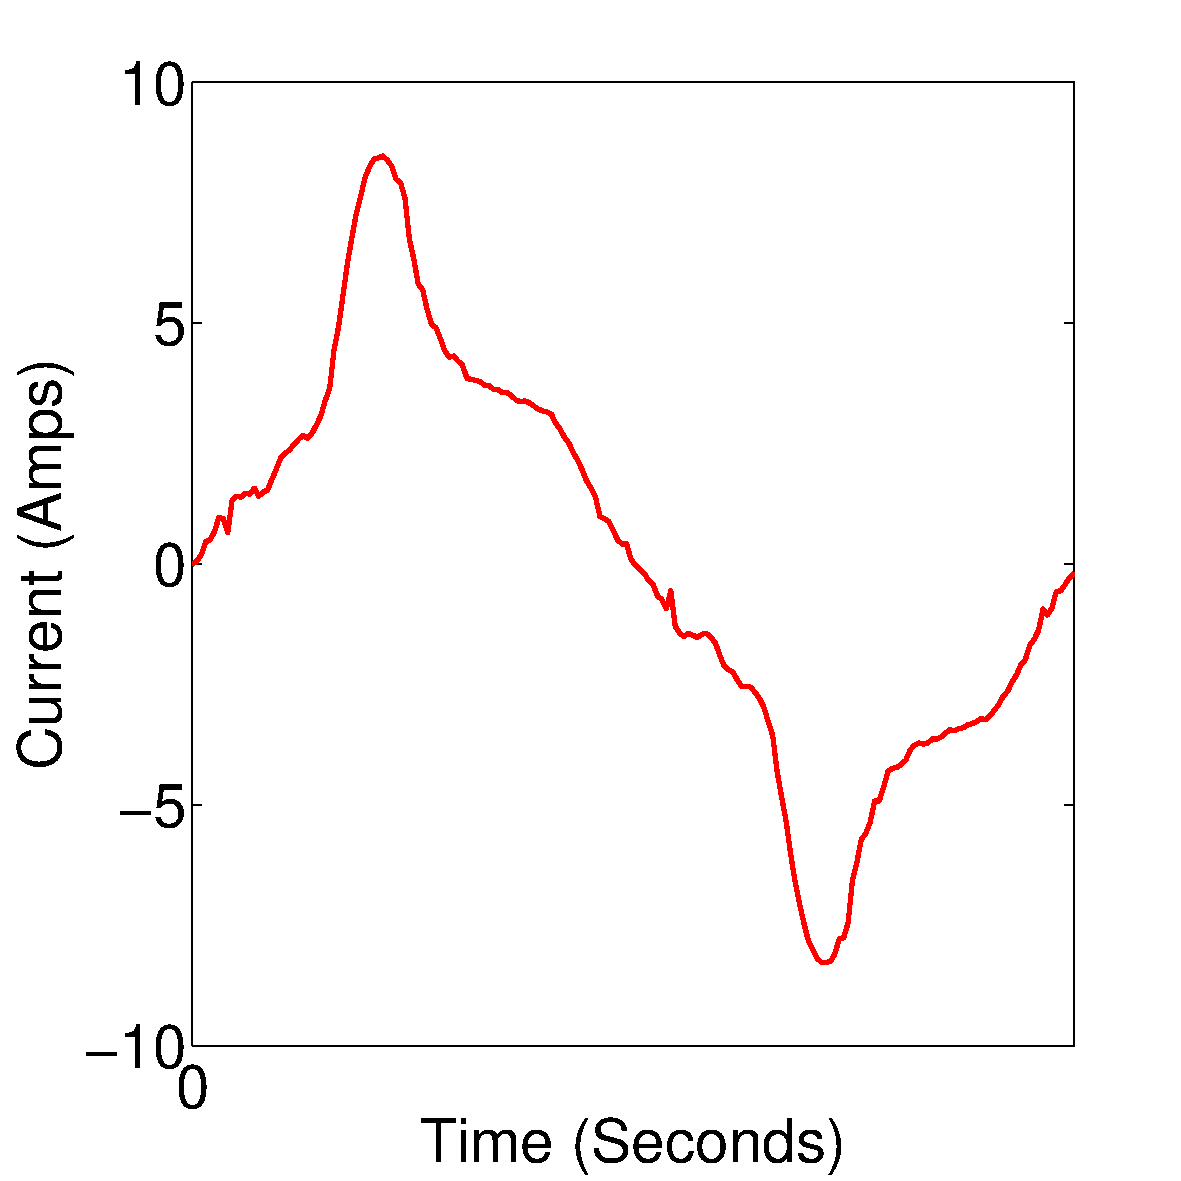
\includegraphics[width=0.4\textwidth,height=0.3\textheight]{figs/Circuit4TransientSingle.pdf} \hspace{1em}&
    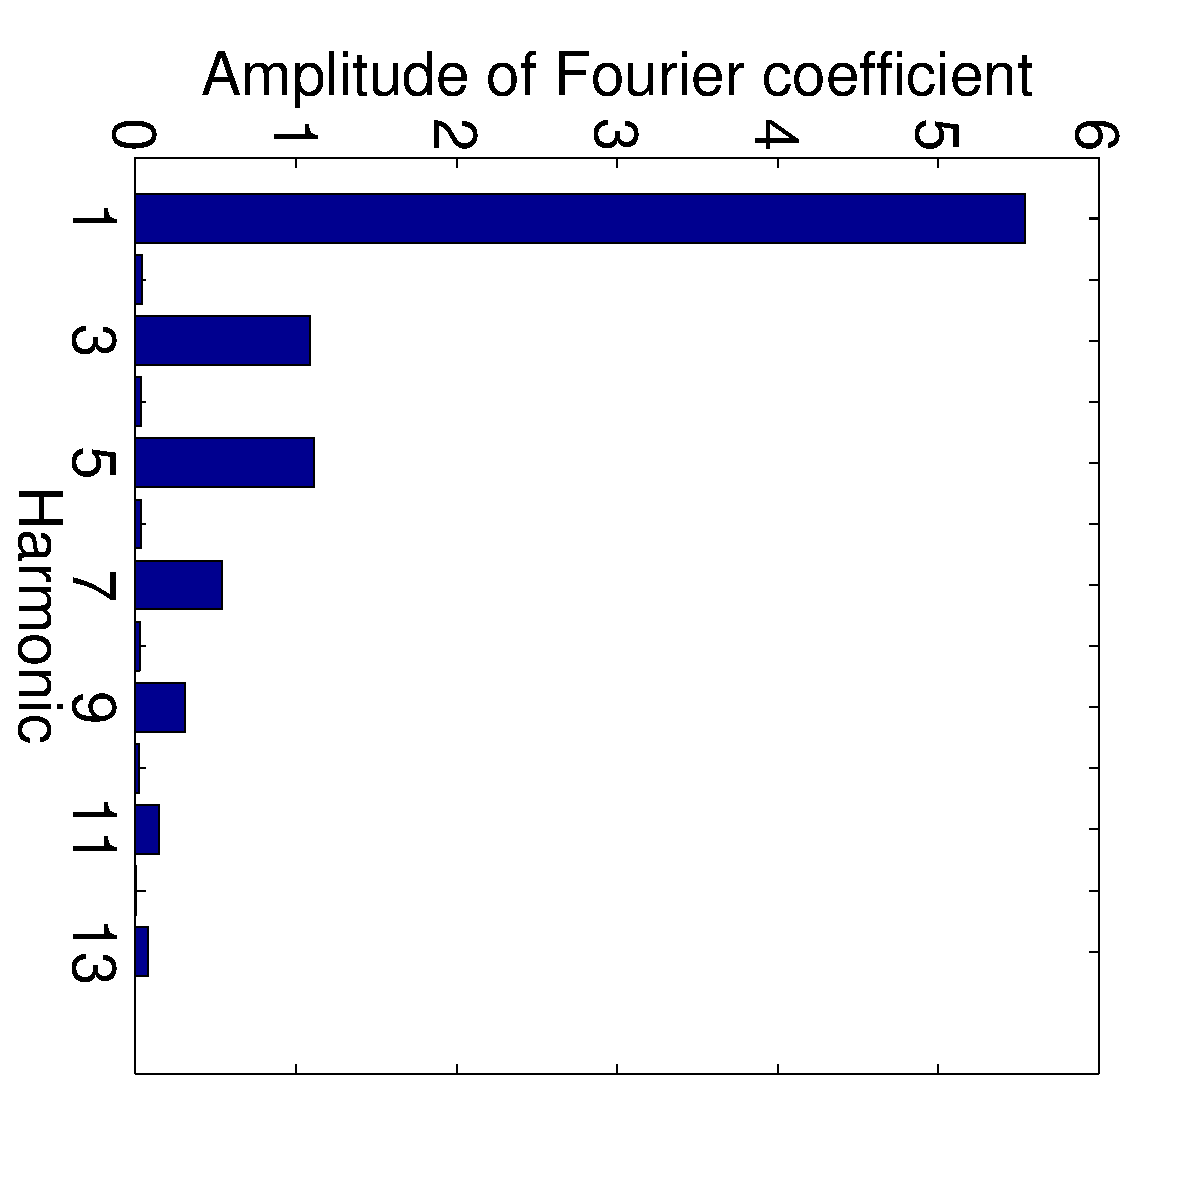
\includegraphics[width=0.4\textwidth,height=0.3\textheight,angle=90]{figs/circuit4TransientFFT.pdf} \tabularnewline
    (a) & (b)\tabularnewline
    \end{tabular}
    }
	\caption{Circuit 4 (a) Current Waveform and (b) Harmonics.}
	\label{fig_harmonicsexample}
\end{figure*}

%\begin{figure}[ht]
%\centering
%\includegraphics[width=3.2in]{figs/harmonicsexample.pdf}
%\caption{Harmonics (courtesy: \cite{eebook}).}
%\label{fig_harmonicsexample}
%\end{figure}
\begin{figure*}[h]
	\centering{
    \begin{tabular}{cc}	
	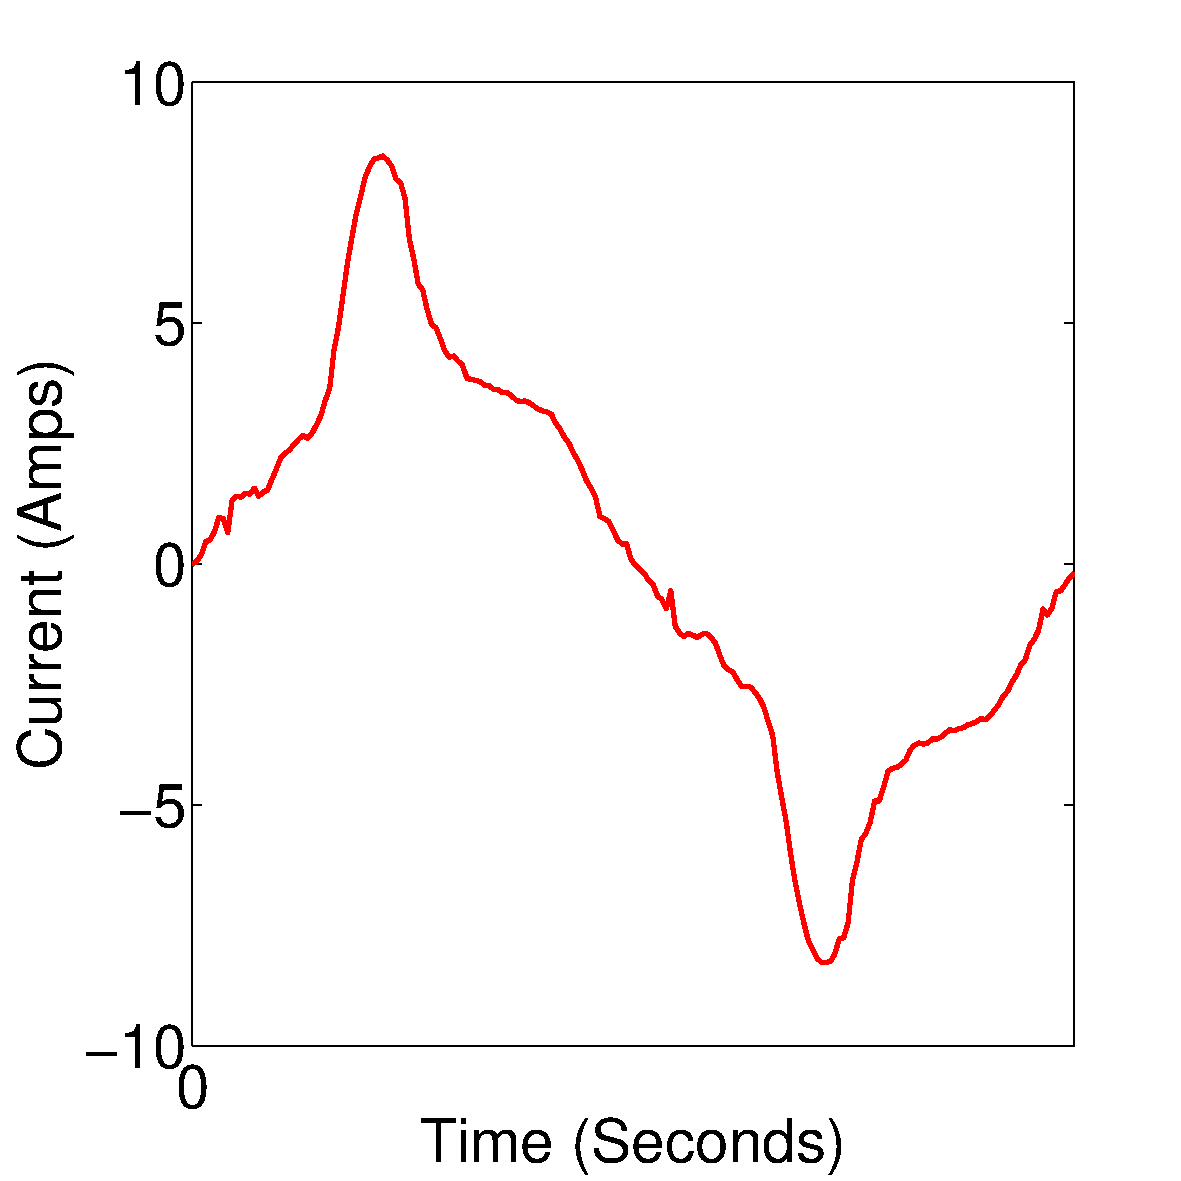
\includegraphics[width=0.4\textwidth,height=0.3\textheight]{figs/Circuit4TransientSingle.pdf} \hspace{1em}&
    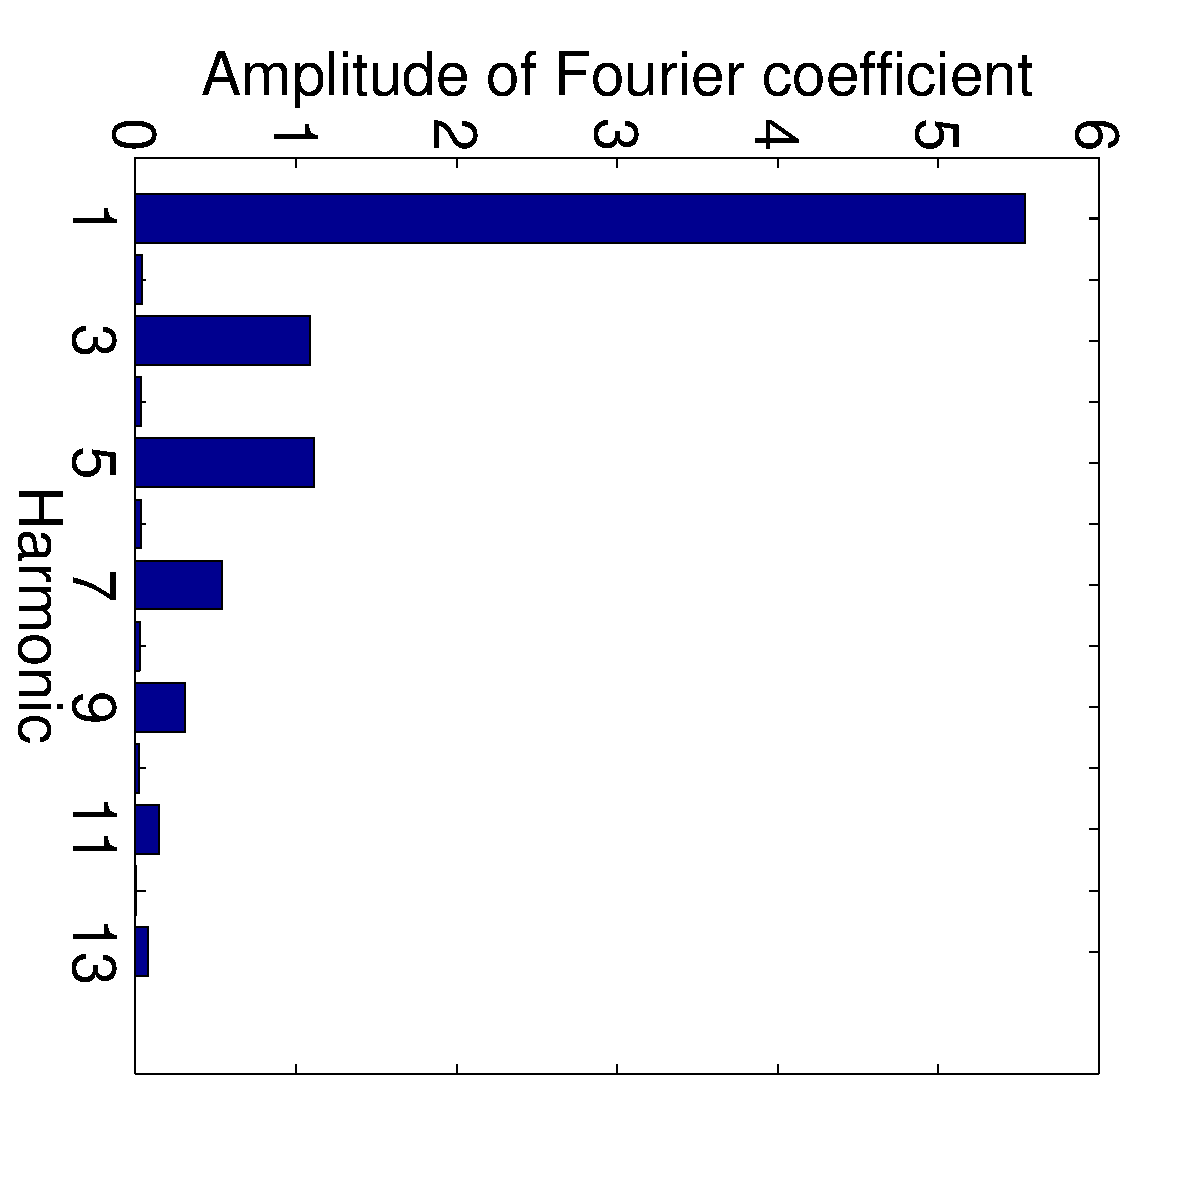
\includegraphics[width=0.4\textwidth,height=0.3\textheight,angle=90]{figs/circuit4TransientFFT.pdf} \tabularnewline
    (a) & (b)\tabularnewline
    \end{tabular}
    }
	\caption{Circuit 4 (a) Current Waveform and (b) Harmonics.}
	\label{fig_harmonicsexample}
\end{figure*}

%\begin{figure}[ht]
%\centering
%\includegraphics[width=3.2in]{figs/harmonicsexample.pdf}
%\caption{Harmonics (courtesy: \cite{eebook}).}
%\label{fig_harmonicsexample}
%\end{figure}
\begin{figure*}[h]
	\centering{
    \begin{tabular}{cc}	
	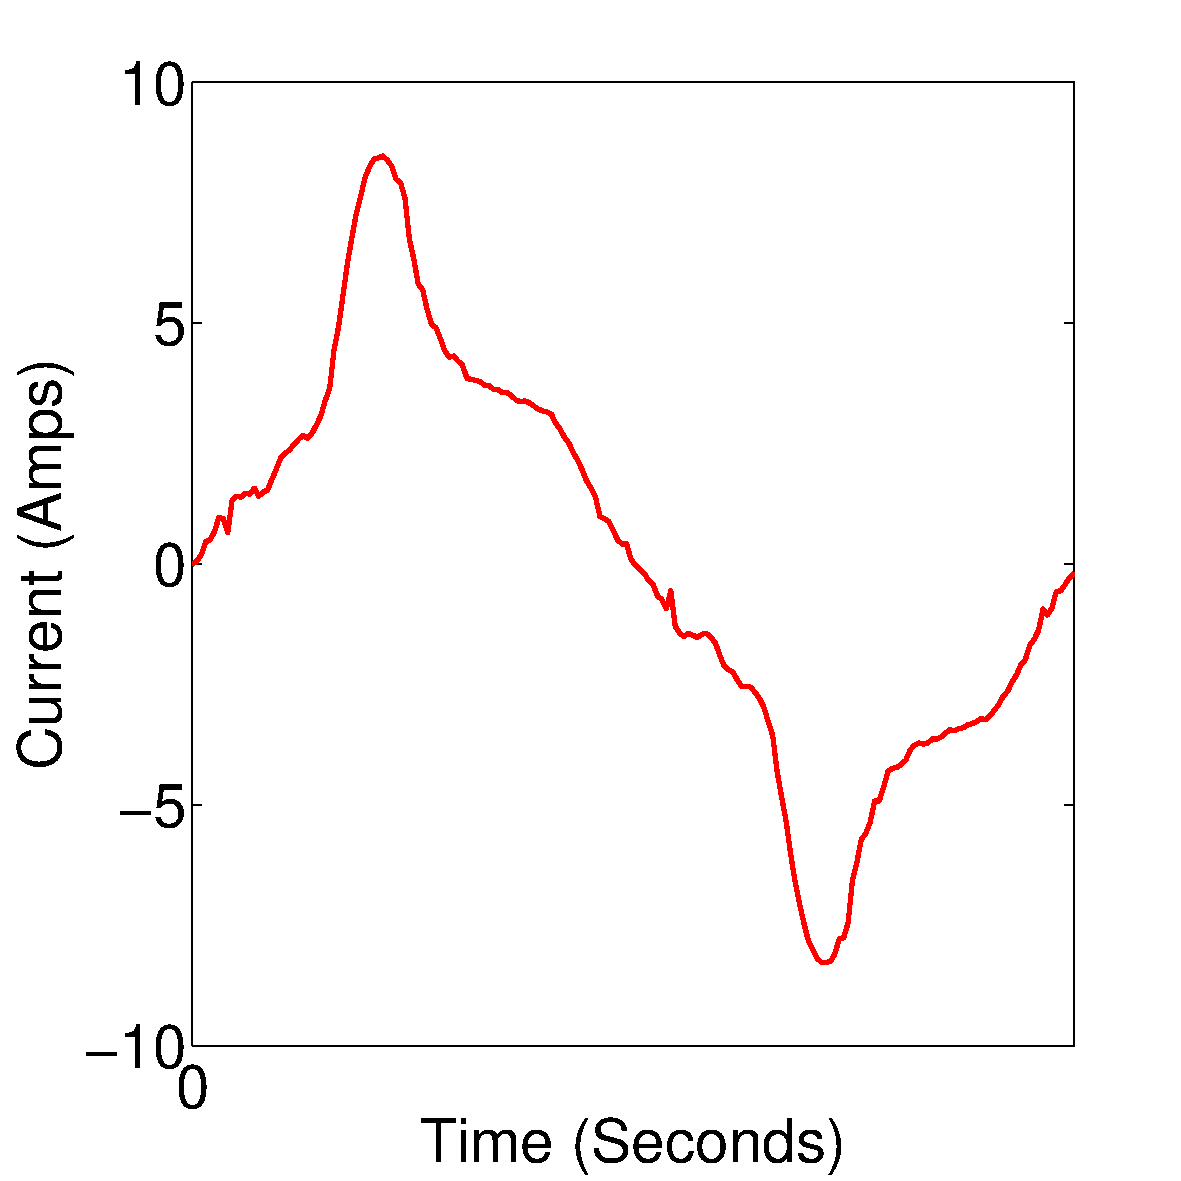
\includegraphics[width=0.4\textwidth,height=0.3\textheight]{figs/Circuit4TransientSingle.pdf} \hspace{1em}&
    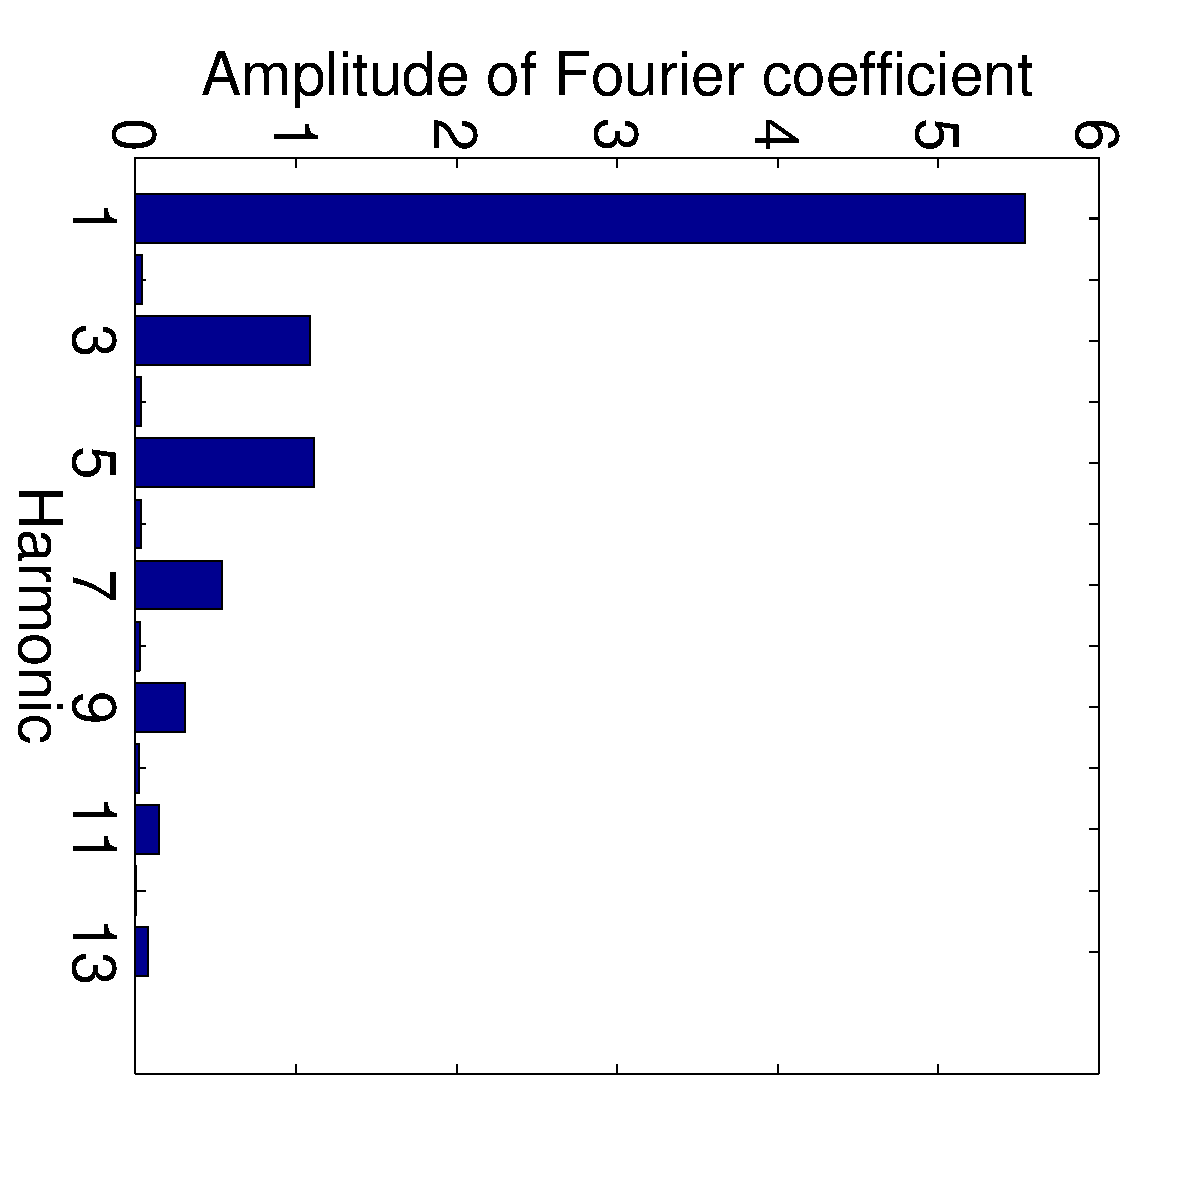
\includegraphics[width=0.4\textwidth,height=0.3\textheight,angle=90]{figs/circuit4TransientFFT.pdf} \tabularnewline
    (a) & (b)\tabularnewline
    \end{tabular}
    }
	\caption{Circuit 4 (a) Current Waveform and (b) Harmonics.}
	\label{fig_harmonicsexample}
\end{figure*}

%\begin{figure}[ht]
%\centering
%\includegraphics[width=3.2in]{figs/harmonicsexample.pdf}
%\caption{Harmonics (courtesy: \cite{eebook}).}
%\label{fig_harmonicsexample}
%\end{figure}
\begin{figure*}[h]
	\centering{
    \begin{tabular}{cc}	
	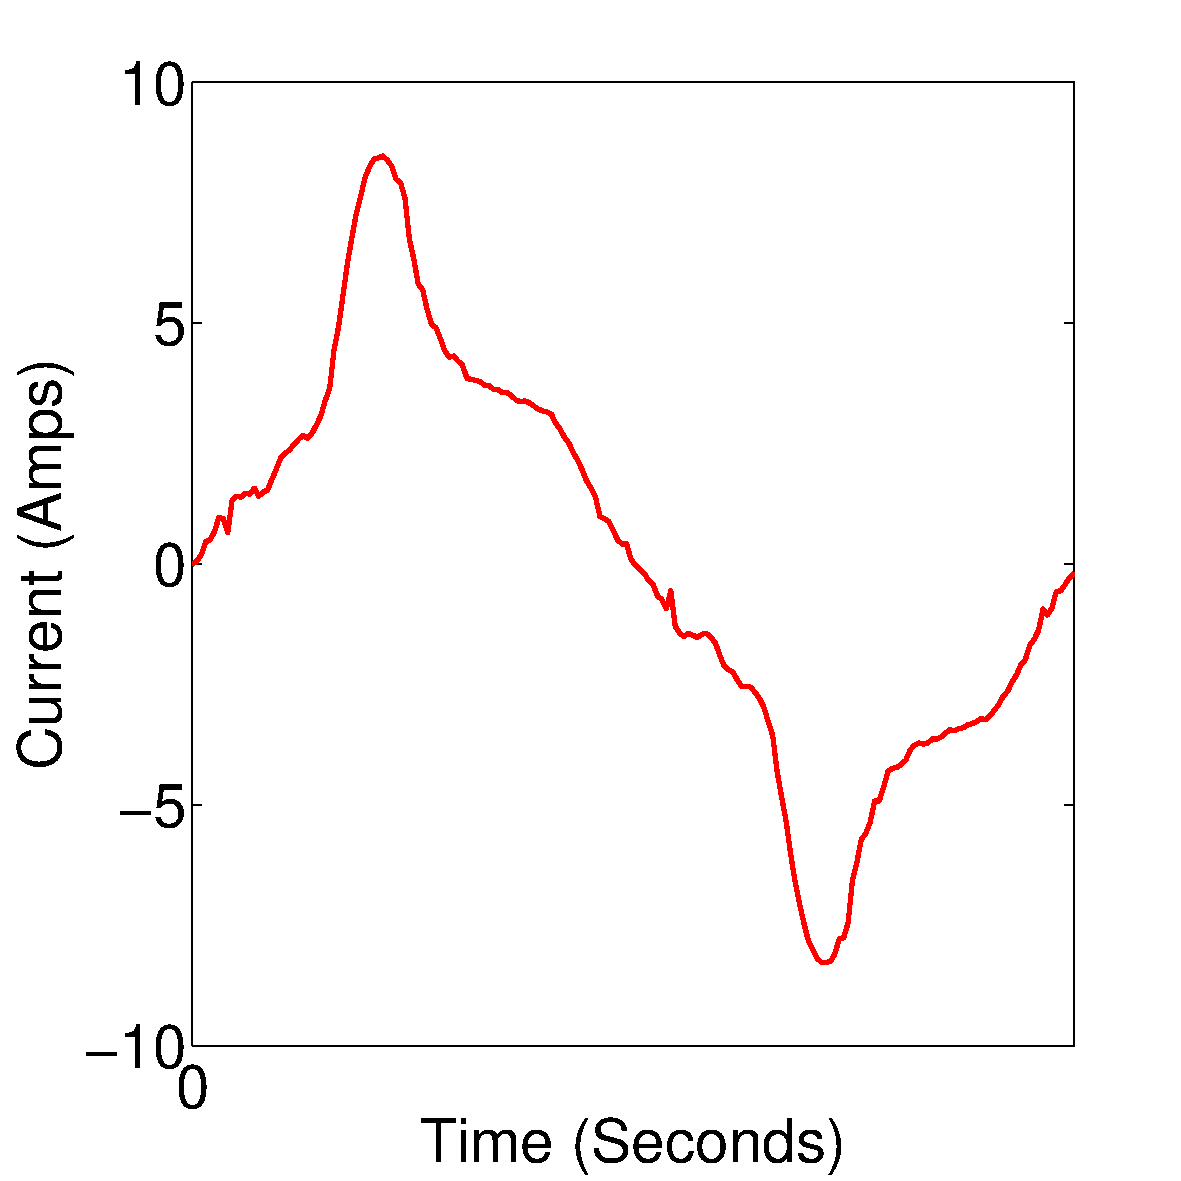
\includegraphics[width=0.4\textwidth,height=0.3\textheight]{figs/Circuit4TransientSingle.pdf} \hspace{1em}&
    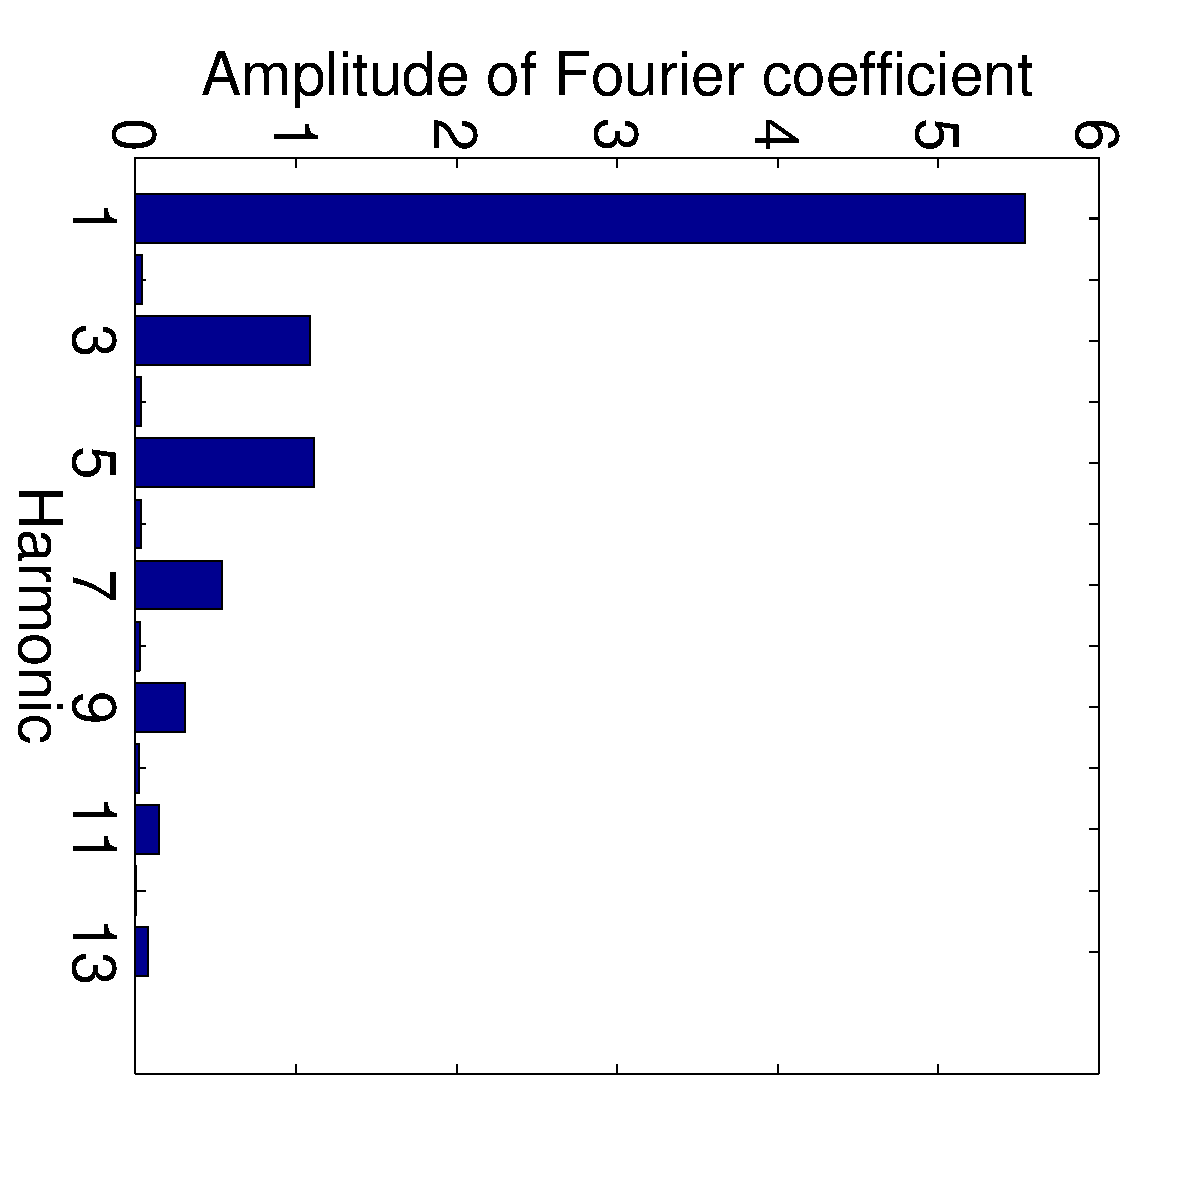
\includegraphics[width=0.4\textwidth,height=0.3\textheight,angle=90]{figs/circuit4TransientFFT.pdf} \tabularnewline
    (a) & (b)\tabularnewline
    \end{tabular}
    }
	\caption{Circuit 4 (a) Current Waveform and (b) Harmonics.}
	\label{fig_harmonicsexample}
\end{figure*}
